\chapter{Experiments and results}

\section{Dataset}

The dataset is composed of video acquired from smartphones and tablets with operating system \emph{Android} and \emph{iOS}. 
Videos that have an \emph{Android} acquisition device have a file container that follows the standard of the MP4 \cite{mp4} file format while videos that have an \emph{iOS} acquisition device have a file container that follows the standard of the MOV file format \cite{mov}.
The full list of devices of the dataset can be seen from Table \ref{devices}. 

\begin{table}[]
\centering
\begin{tabular}{|l|l|l|l|}
\hline
\textbf{OS}       & \textbf{BRAND}    & \textbf{MODEL}             & \textbf{\#}			 \\ \hline
Android &         &                   & 150         \\ \hline
        & Samsung &                   & 132         \\ \hline
        &         & Galaxy S3         & 18          \\ \hline
        &         & Galaxy S3 mini    & 36          \\ \hline
        &         & Galaxy S4 mini    & 18          \\ \hline
        &         & Galaxy Tab 3      & 36          \\ \hline
        &         & Galaxy Tab A      & 9           \\ \hline
        &         & Galaxy Trend Plus & 15          \\ \hline
        & Huawei  &                   & 18          \\ \hline
        &         & G6                & 18          \\ \hline
iOS     &         &                   & 110         \\ \hline
        & Apple   &                   & 110         \\ \hline
        &         & iPad 2            & 15          \\ \hline
        &         & iPad mini         & 15          \\ \hline
        &         & iPhone 4S         & 14          \\ \hline
        &         & iPhone 5C         & 18          \\ \hline
        &         & iPhone 5          & 31          \\ \hline
        &         & iPhone 6          & 17          \\ \hline
        &         &                   & 260         \\ \hline

\end{tabular}
\caption{The list of devices in the dataset divided by operating system, brand and model.}
\label{devices}
\end{table}

Each video of the dataset has also been modified thought different means:

\begin{itemize}
\item videos that have been uploaded and then downloaded from 	\emph{Youtube}.
\item videos that have been modified using the software tool \emph{Ffmpeg} \cite{ffmpeg}.
\item videos that have been modified using the software tool \emph{Exiftool} \cite{exiftool}.
\end{itemize}

\section{Integrity Verification based on File Container}

In order to determine how our approach performs with regard to Integrity Verification we have set up some experiments. As mentioned above, the videos of the dataset have also been modified through different means, thus losing their integrity. In these experiments we check whether the information of the file containers are sufficient to tell the original videos and the modified ones apart.

The tools that we have used to modify the videos are \emph{Ffmpeg} and \emph{Exiftool}. The modification we have made are as minimal as the tools allow.

In general the experiments have been performed as follow. Given a set of videos $(x_{1},\ldots,x_{n}) \in C_{i}$, with $C_{i}$ a certain device, we have generated the corresponding set of minimally processed videos $(\overline{x_{1}},\ldots,\overline{x_{n}})$ using a certain tool. For each couple of videos $(x_{i}, x_{j})$ of the same device we have computed the differences using the \emph{compare} feature of the Video Format Tool. The differences are then divided by the total number of attributes in the file container that is taken as reference (as explained in Section 3.2), giving us a distance between videos represented as a number between 0 and 1. These distances tell us how much the videos of the same device differ. Then we compute the difference for each couple of $(x_{i}, \overline{x_{j}})$ and for each couple $(\overline{x_{i}}, x_{j})$ to determine how much the original videos differ from the processed ones. We repeat this operation for each device in our dataset.

At the end of the computation we will have a sequence of distances. To each distance we associate a label, 1 when it corresponds to a comparison between original videos and 0 when it corresponds to a comparison between an original video and a processed one.

Then, we determine a threshold that is able to correctly separate the two classes. The first class is composed by the distances between original videos of the same devices; the second is composed by the distances between original and processed videos of the same devices. Using a ROC curve, we illustrate the performance of this simple binary classifier system as the discrimination threshold varies.

Once the best threshold that maximizes the ratios between true positive rate (TPR) and false positive rate (FPR) is chosen, we compute the accuracy as:

\begin{equation}\label{eq:accuracy}
ACC = \dfrac{TPR + (1 - FPR)}{2}
\end{equation}

\subsection{Ffmpeg}

The \emph{Ffmpeg} tool is a cross-platform software to record, modify, convert and stream audio and video. The videos in our dataset have been processed so that, without re-encoding, each video has been truncated after a certain amount of frames, using the following command:

\begin{lstlisting}
ffmpeg -i input.mp4 -ss 00:00:00 -t 00:00:10 -acodec copy -vcodec copy output.mp4
\end{lstlisting}

The distances have been computed as explained above. As we can see from Fig. \ref{fig:ffmpeg-hist}, the two classes, i.e. the set of distances between original videos and the set of distances between original and processed videos, are greatly separated. This fact means that there is an ample range of threshold values for which the accuracy is maximized. For this case, we have a max accuracy of 100\% for a range of threshold values between 0.11 and 0.66.

\begin{figure}
  \centering
  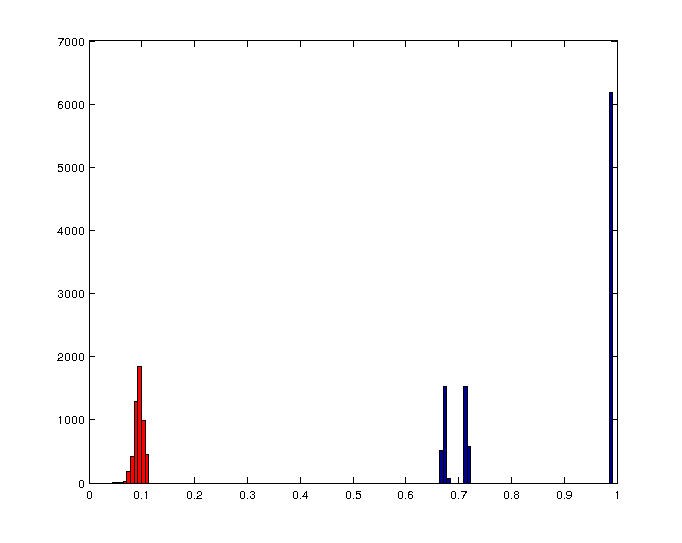
\includegraphics[width=1\textwidth]{ffmpeg-hist}
  \caption{The distribution of the distances between original videos (in red) and the distribution of the distances between original videos and videos processed with ffmpeg (in blue).}\label{fig:ffmpeg-hist}
\end{figure}

The results show that when a video is processed by \emph{Ffmpeg} copying the video stream without re-encoding is enough to greatly alter the file container structure. In fact, original videos from the same device do not differ more than the 11\% in their file containers while the difference between original and processed videos from the same device is at least 66\%.

\subsection{Exiftool}

\emph{Exiftool} is a command line application for reading, writing and editing metadata information in a variety of media files. With this tool, we have changed all the time related information of our dataset videos, using the following command:

\begin{lstlisting}
exiftool "-AllDates=1986:11:05 12:00:00" "input.mp4"
\end{lstlisting}

Since we are modifying attributes of the file container that are specific to each unique video, we did not expect this test to perform well. The results are in agreement with this assumption. The changes that \emph{Exiftool} does on a file container are minimal; it just adds a new box at the end of the file, leaving the rest of the structure untouched. As we can see from Fig. \ref{fig:exifaal-hist}, it is not possible to find a threshold that correctly separates the two classes of the binary problem.

\begin{figure}
  \centering
  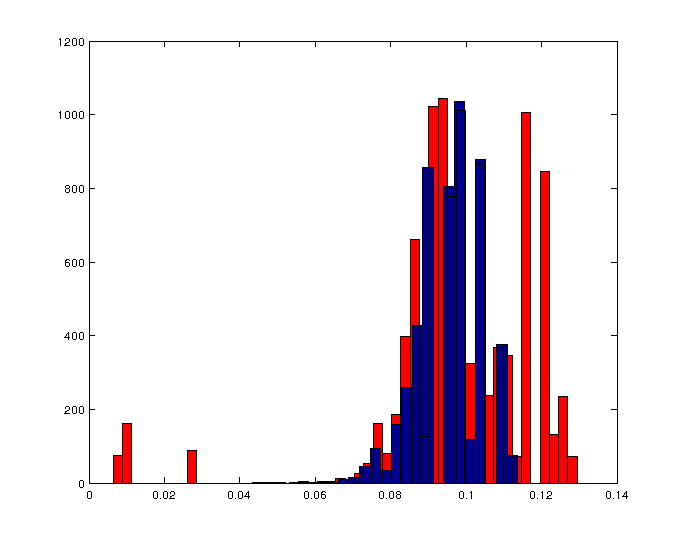
\includegraphics[width=1\textwidth]{exifall-hist}
  \caption{The distribution of the distances between original videos (in red) and the distribution of the distances between original videos and videos processed with exiftool (in blue) overlap.}\label{fig:exifaal-hist}
\end{figure}

\begin{figure}
  \centering
  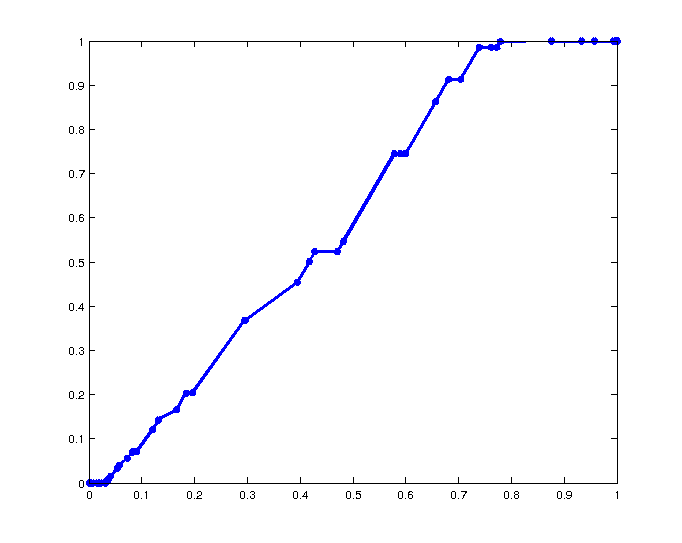
\includegraphics[width=1\textwidth]{exifall-plot}
  \caption{The ROC curve for the experiment with Exiftool shows how the TPR and FPR varies when changing the threshold value.}\label{fig:brand-roc}
\end{figure}

This situation happens because, when we consider all devices, the distances between original videos of the same class for the \emph{Android} devices and for the \emph{iOS} devices have different average values. The box that \emph{Exiftool} inserts to the file container for each processed videos adds a constant number of differences for every comparison. This causes the curve associated to the distances between original and processed videos of \emph{Android} devices to overlap the curve associated to the distances between original videos for \emph{iOS} devices.

However, we noticed that the differences between original videos of the same device regard attributes that are unique to each video, such as \emph{creationTime}, \emph{modificationTime}, \emph{size}, etc. We decided to solve this issue by dynamically build a set composed by attributes whose values are unique to each video for every devices. During the comparison, we will ignore the differences caused by such attributes because their values are not specific to a certain device but to each video.

Without considering such attributes, we are able to separate the two classes with a max accuracy of 100\% using a threshold of 0.001. This result means that even a 0.1\% difference in the file containers is enough to determine if a video was processed by \emph{Exiftool}, if we do not consider attributes that are unique to each video.

\section{Application on Social Network}

We have also applied our method to videos that come from a Social Network, specifically from \emph{Youtube}. The videos of our dataset have been uploaded and then downloaded from \emph{Youtube}.

The experiments have been carried out similarly to the ones for the Integrity Verification. However, we want to determine if videos from \emph{Youtube} are sufficiently similar to be able to distinguish a video that come directly from a source device from a video of that source device that have been subsequently uploaded and downloaded from \emph{Youtube}.

\begin{figure}
  \centering
  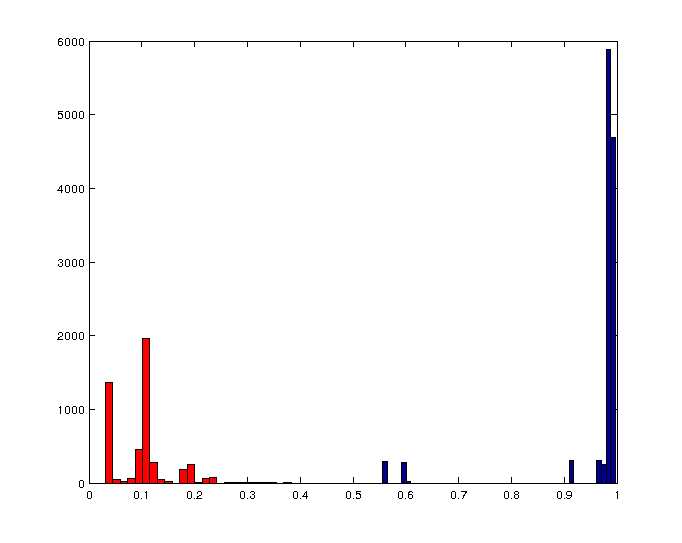
\includegraphics[width=1\textwidth]{youtube-hist}
  \caption{The distribution of the distances between \emph{Youtube} videos (in red) and the distribution of the distances between \emph{Youtube} videos and original videos (in blue).}\label{fig:youtube-hist}
\end{figure}

As can be seen from Fig. \ref{fig:youtube-hist}, the values representing the distances between \emph{Youtube} videos and the ones representing the distances between original and \emph{Youtube} videos are greatly separated. We obtain a max accuracy of 100\% with a range of threshold values between 0.39 and 0.55. Similar as before, \emph{Youtube} videos differ for a max of 39\% of their file containers while the difference between \emph{Youtube} and original videos differ of at least 55\%.

\section{Source Identification based on File Container}

This section will describe the experiments run to assess the accuracy of our approach with regard to Source Identification. For each video of the test set we compute the likelihood ratio with respect to every class of device in the training set. 

When computing the likelihood, the attributes that pertain to the videos and not to the class, as explained previously, will be ignored.

After all the computation have finished, we will obtain a vector of likelihood ratios. To each likelihood ratio we need to associate a label accordingly to the class of the test video and the class for which the likelihood have been computed. The label will be 1 if the tested class is the exact brand and model or only the exact brand of test video; it will be 0 otherwise.

Using the ROC curve, we determine the threshold value for the likelihood ratio that maximizes the accuracy, computed as \ref{eq:accuracy}.

We consider separately the classes that specify only the brand of devices and the classes that refer to brands and models, taking into account both manual and automatic mode.

For the automatic mode, we measure the precision of our system. Since for this mode, as it works in the web application, no assumption about the class is made, we return a list of classes in decreasing order of likelihood ratio. To determine how precise our approach is, we check whether the correct class is in first position (TOP 1), in the first three positions (TOP 3), and in the first five positions (TOP 5). When considering brands, the precision is only computed checking if the correct class is in first position, due to the limited number of brands available in our dataset.

\subsubsection*{Brands}

We can see from the ROC curve shown in Fig. \ref{fig:brand-roc} how the TPR and the FPR change when the threshold varies.
For manual mode, we obtain a maximum accuracy of 98.08\% with a range of likelihood values between -12 and 14, determined using the results from the ROC curve.

\begin{figure}
  \centering
  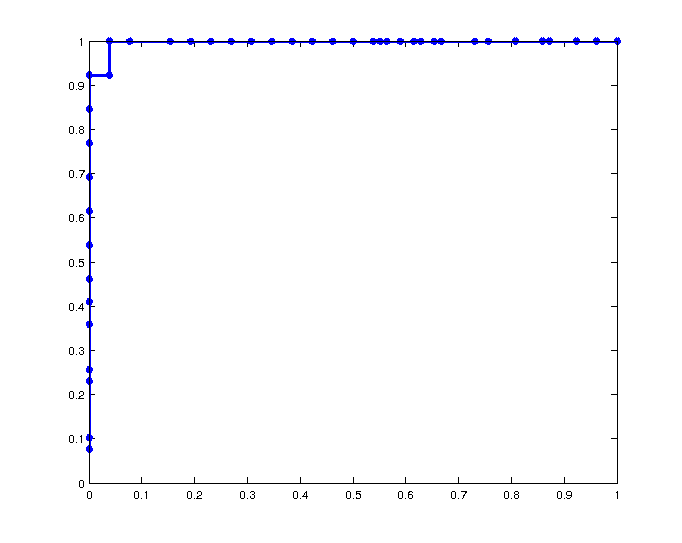
\includegraphics[width=1\textwidth]{brandig-plot}
  \caption{The ROC curve for the experiment with brands classes shows how the TPR and FPR varies when changing the threshold value.}\label{fig:brand-roc}
\end{figure}

With regard to precision, 92\% of the time the first result returned by automatic mode is the correct one. For this case, the results can also be visualized in Fig. \ref{fig:brand-conf} where it is shown the confusion matrix. With the confusion matrix we are able to see in which direction the misclassifications happened. We can see that the only errors happened because some Samsung devices are classified as Huawei devices. 

\begin{figure}
  \centering
  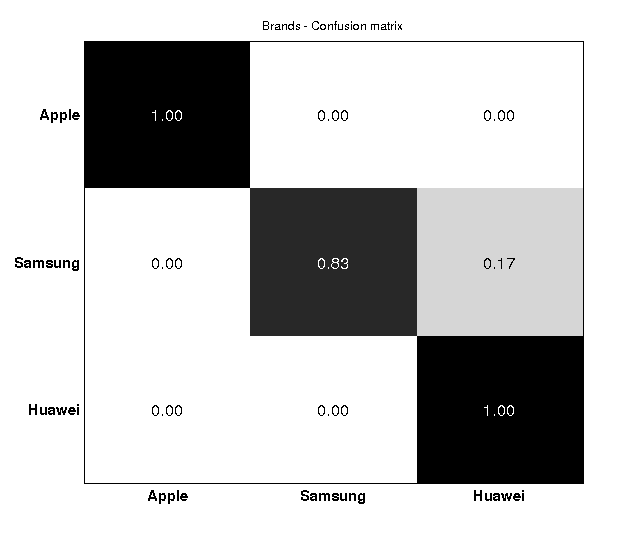
\includegraphics[width=0.7\textwidth]{conf-brands}
  \caption{Confusion matrix that shows how the test videos are classified with regard to brands.}\label{fig:brand-conf}
\end{figure}

\subsubsection*{Brands and Models}

We consider class for which both brand and model are specified. 

For the manual mode, we obtain a maximum accuracy of 97.54\% for a range of likelihood values between 3 and 4. The ROC curve can be seen in Fig. \ref{fig:model-roc}.  The range of best threshold values is not centered in 0 because of similarities between certain models that causes some errors. In fact, with a threshold value of 0, the accuracy drops to 96.79\%.

\begin{figure}
  \centering
  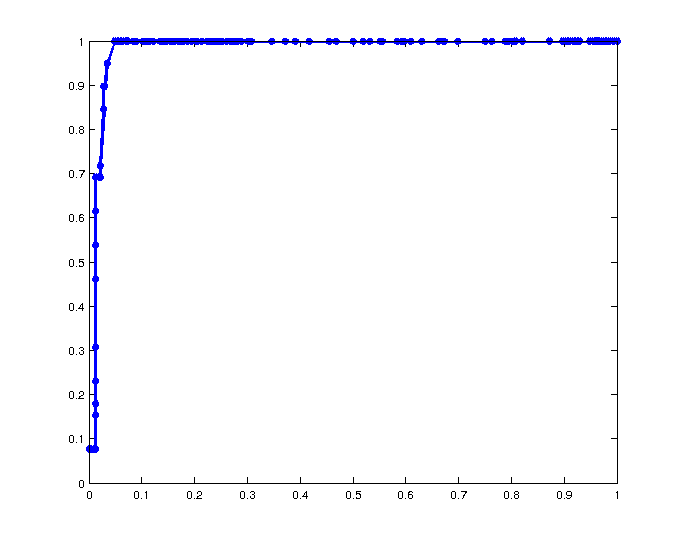
\includegraphics[width=1\textwidth]{modelig-plot}
  \caption{The ROC curve for the experiment with brands and models classes shows how the TPR and FPR varies when changing the threshold value.}\label{fig:model-roc}
\end{figure}

For the automatic mode, we determine the precision as explained before. We have that 84.62\% of the time the first result, i.e. the result with the highest likelihood ratio, is also the correct one. Instead, we get a precision of 100\% for both TOP 3 and TOP 5: the correct brand and model class is at least in third position in terms of likelihood.